\documentclass[a4paper,11pt]{article}

\usepackage{geometry}
\geometry{margin=0.8in}

\usepackage{amsmath}
\usepackage{amssymb}
\usepackage{mathtools}
\usepackage{graphicx}
\usepackage{xcolor}

\usepackage{siunitx}
\sisetup{detect-all}

\usepackage[colorlinks=true,linkcolor=blue3,citecolor=blue3,urlcolor=blue3]{hyperref}

\usepackage{cleveref}

\usepackage{tcolorbox}
\tcbuselibrary{skins,breakable}

\usepackage{booktabs}
\usepackage{enumitem}
\usepackage{tikz}

\definecolor{blue3}{RGB}{0,0,180}
\definecolor{green3}{RGB}{0,120,0}
\definecolor{orange3}{RGB}{200,100,0}
\definecolor{red3}{RGB}{180,0,0}

\newtcolorbox{derivationbox}[1][]{
    colback=blue!10,
    colframe=blue3,
    coltitle=blue3,
    title={Derivation:},
    fonttitle=\bfseries,
    #1
}

\newtcolorbox{resultbox}[1][]{
    colback=green!10,
    colframe=green3,
    coltitle=green3,
    title={Result Summary:},
    fonttitle=\bfseries,
    #1
}

\newtcolorbox{warningbox}[1][]{
    colback=orange!10,
    colframe=orange3,
    coltitle=orange3,
    title={Warning:},
    fonttitle=\bfseries,
    #1
}

\newcommand{\ktilde}{\tilde{k}}
\newcommand{\ytilde}{\tilde{y}}
\newcommand{\ctilde}{\tilde{c}}
\newcommand{\khat}{\hat{k}}
\newcommand{\ychat}{\hat{y}}
\newcommand{\chat}{\hat{c}}
\newcommand{\diff}{\mathrm{d}}
\newcommand{\ubar}[1]{\underline{#1}}

\title{\textbf{Ramsey/Cass/Koopmans Model Cheatsheet}}
\author{Macroeconomics I - Lecture 2}
\date{UPF, CREi, BSE \& CEPR}

\begin{document}

\maketitle

\clearpage

\section*{Notation and Definitions}

\subsection*{Aggregate Variables}
\begin{itemize}
    \item $K_t$: Aggregate capital stock
    \item $L_t$: Aggregate labor (population)
    \item $Y_t$: Aggregate output
    \item $A_t \equiv B_t$: Technology level (labor-augmenting, $\dot{A}/A = x$)
    \item $C_t$: Aggregate consumption
    \item $N_t$: Family size, $N_t = N_0 e^{nt}$ with $N_0 = 1$
\end{itemize}

\subsection*{Per Worker Variables ($k = K/L$, $y = Y/L$, $c = C/L$)}
\begin{itemize}
    \item $k_t = K_t / L_t$: Capital per worker
    \item $y_t = Y_t / L_t$: Output per worker
    \item $c_t = C_t / L_t$: Consumption per worker
\end{itemize}

\subsection*{Per Effective Worker Variables ($\tilde{k} = K/(AL)$, etc.)}
\begin{itemize}
    \item $\ktilde_t = K_t / (A_t L_t)$: Capital per effective worker
    \item $\ytilde_t = Y_t / (A_t L_t)$: Output per effective worker
    \item $\ctilde_t = C_t / (A_t L_t)$: Consumption per effective worker
    \item Alternative notation: $\khat_t$, $\ychat_t$, $\chat_t$ (used in lecture)
\end{itemize}

\subsection*{Parameters}
\begin{itemize}
    \item $n$: Population growth rate
    \item $x$: Technology (TFP) growth rate
    \item $\delta$: Depreciation rate
    \item $\rho$: Subjective discount rate ($\rho > 0$)
    \item $\sigma$: CRRA curvature parameter ($-\frac{u_{cc}c}{u_c}$)
    \item $s$: Savings rate (endogenous in Ramsey, exogenous in Solow)
\end{itemize}

\clearpage

\section*{Model Setup}

\subsection*{Environment}
\begin{itemize}
    \item Single homogeneous good (consumed or invested)
    \item Closed economy
    \item Exogenous population growth: $n$
    \item Exogenous technology growth: $x$ (labor-augmenting)
    \item Representative household and firm
    \item Three competitive markets: capital, labor, final good
\end{itemize}

\subsection*{Firm Problem}
The representative firm maximizes profits:
\[
\Pi_t = F(K_t, A_t L_t) - (r_t + \delta)K_t - w_t L_t
\]
\begin{resultbox}
\[
F_K(K_t, A_t L_t) = r_t + \delta \quad \text{(marginal product of capital)}
\]
\[
F_L(K_t, A_t L_t) = w_t \quad \text{(marginal product of labor)}
\]
\end{resultbox}

Using per-effective units: $y = f(k)$ where $f(k) = F(k, 1)$
\[
f'(\ktilde) = r + \delta
\]

\subsection*{Household Budget Constraint}
Per worker form:
\[
c_t + \dot{a}_t + n a_t = w_t + r_t a_t
\]
where $a_t = A_t / L_t$ (assets per worker).

\clearpage

\section*{Derivation: Household Optimization}

\subsection*{Household Problem}
Maximize lifetime utility:
\[
\max_{\{c_t, a_t\}} \int_0^\infty u(c_t) e^{-(\rho-n)t} \, \diff t
\]
Subject to:
\[
c_t + \dot{a}_t + n a_t \le w_t + r_t a_t, \quad a_0 \text{ given}
\]
No-Ponzi Game: $\lim_{t\to\infty} a_t e^{-\int_0^t (r_s-n) \diff s} \ge 0$

\subsection*{Current-Value Hamiltonian Setup}
\[
\mathcal{H} = u(c_t) + \nu_t [w_t + (r_t - n)a_t - c_t]
\]
where $\nu_t$ is the co-state (shadow price of assets).

\begin{derivationbox}{First-Order Conditions}
\textbf{Control variable ($c$):}
\[
\mathcal{H}_c = 0 \Rightarrow \nu_t = u_c(c_t)
\]

\textbf{State variable ($a$):}
\[
\mathcal{H}_a = \rho \nu_t - \dot{\nu}_t \Rightarrow \dot{\nu}_t = -(r_t - n)\nu_t
\]

\textbf{State equation:}
\[
\mathcal{H}_\nu = \dot{a}_t = w_t + (r_t - n)a_t - c_t
\]
\end{derivationbox}

\subsection*{Euler Equation Derivation}
Take logs of $\nu_t = u_c(c_t)$:
\[
\log \nu_t = \log u_c(c_t) - (\rho - n)t
\]

Differentiate with respect to $t$:
\[
\frac{\dot{\nu}_t}{\nu_t} = \frac{u_{cc} \dot{c}_t}{u_c} - (\rho - n)
\]

Substitute $\dot{\nu}_t = -(r_t - n)\nu_t$:
\[
-(r_t - n) = \frac{u_{cc} c_t}{u_c} \frac{\dot{c}_t}{c_t} - (\rho - n)
\]

Rearrange to obtain:

\begin{resultbox}
\[
\frac{\dot{c}_t}{c_t} = \left[ -\frac{u_{cc}(c_t) c_t}{u_c(c_t)} \right]^{-1} (r_t - \rho)
\tag{Euler Equation (General)}
\]
\end{resultbox}

For CRRA utility $u(c) = \frac{c^{1-\sigma} - 1}{1-\sigma}$:

\begin{resultbox}
\[
\boxed{\frac{\dot{c}_t}{c_t} = \frac{1}{\sigma}(r_t - \rho)}
\tag{Euler Equation (CRRA)}
\]
\end{resultbox}

Intuition: Households save more if $r > \rho$ (return exceeds discount rate). Higher $\sigma$ reduces the response to interest rate changes.

\clearpage

\section*{Equilibrium and Dynamic System}

\subsection*{Market Clearing}
\begin{itemize}
    \item Labor market: $L_t = N_t$
    \item Asset market: $K_t = N_t a_t$
\end{itemize}

\subsection*{Aggregate Resource Constraint}
From household BC and market clearing:
\[
\dot{k}_t = y_t - c_t - (n + \delta)k_t
\tag{Per worker}
\]

Per-effective-worker form:
\[
\dot{\ktilde}_t = f(\ktilde_t) - \ctilde_t - (n + x + \delta)\ktilde_t
\tag{Per effective}
\]

\subsection*{Complete Dynamic System}
\[
\begin{aligned}
\dot{\ktilde} &= f(\ktilde) - \ctilde - (n + x + \delta)\ktilde \\
\frac{\dot{\ctilde}}{\ctilde} + x &= \frac{1}{\sigma}(f'(\ktilde) - \delta - \rho)
\end{aligned}
\]

\clearpage

\section*{Steady State Analysis}

\subsection*{Steady State Conditions}
Set growth rates to zero ($\gamma_{\ktilde} = 0$, $\gamma_{\ctilde} = 0$):

\begin{resultbox}
\[
\ctilde^* = f(\ktilde^*) - (n + x + \delta)\ktilde^* 
\tag{$\dot{\ktilde} = 0$}
\]
\[
f'(\ktilde^*) = \delta + \rho + \sigma x
\tag{Modified Golden Rule}
\]
\end{resultbox}

\subsection*{Cobb-Douglas Case}
Let $f(\ktilde) = \ktilde^\alpha$ with $0 < \alpha < 1$:

\begin{resultbox}
\[
\ktilde^* = \left( \frac{\alpha}{\delta + \rho + \sigma x} \right)^{\frac{1}{1-\alpha}}
\]
\[
\ytilde^* = \left( \frac{\alpha}{\delta + \rho + \sigma x} \right)^{\frac{\alpha}{1-\alpha}}
\]
\[
\ctilde^* = \ytilde^* - (n + x + \delta)\ktilde^*
\]
\end{resultbox}

\subsection*{Golden Rule Comparison}
\begin{itemize}
    \item \textbf{Solow Golden Rule}: $f'(\ktilde_{GR}) = n + x + \delta$
    \item \textbf{Ramsey Modified Golden Rule}: $f'(\ktilde^*) = \delta + \rho + \sigma x$
\end{itemize}

Since $\rho > 0$ and $\sigma > 0$:
\[
f'(\ktilde^*) > f'(\ktilde_{GR}) \Rightarrow \ktilde^* < \ktilde_{GR}
\]

\clearpage

\section*{Phase Diagram and Transitional Dynamics}

\subsection*{Phase Diagram Loci}

\begin{center}
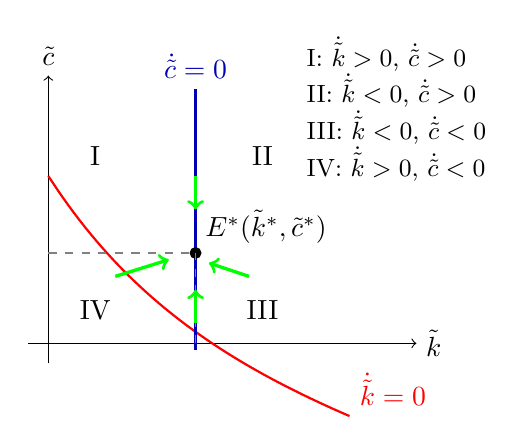
\begin{tikzpicture}[scale=0.85]
    \draw[->] (-0.3,0) -- (5.5,0) node[right] {$\ktilde$};
    \draw[->] (0,-0.3) -- (0,4) node[above] {$\ctilde$};
    
    \draw[domain=0:4.5,smooth,variable=\x,red,thick] 
        plot ({\x},{2.5 * exp(-0.5*\x) - 0.3*\x}) 
        node[above right,red] {$\dot{\ktilde}=0$};
    
    \draw[blue3,thick] (2.2,-0.1) -- (2.2,3.8) node[above,blue3] {$\dot{\ctilde}=0$};
    
    \draw[fill=black] (2.2,1.35) circle (0.08) node[above right] {$E^*(\ktilde^*,\ctilde^*)$};
    
    \draw[dashed,gray] (0,1.35) -- (2.2,1.35);
    \draw[dashed,gray] (2.2,0) -- (2.2,1.35);
    
    \draw[->,green,very thick] (1.0,1.0) -- (1.8,1.25);
    \draw[->,green,very thick] (3.0,1.0) -- (2.4,1.2);
    \draw[->,green,very thick] (2.2,2.5) -- (2.2,2.0);
    \draw[->,green,very thick] (2.2,0.3) -- (2.2,0.8);
    
    \node at (0.7,2.8) {I};
    \node at (3.2,2.8) {II};
    \node at (3.2,0.5) {III};
    \node at (0.7,0.5) {IV};
    
    \node[align=left,font=\small] at (5.2,3.5) {I: $\dot{\ktilde}>0$, $\dot{\ctilde}>0$\\ II: $\dot{\ktilde}<0$, $\dot{\ctilde}>0$\\ III: $\dot{\ktilde}<0$, $\dot{\ctilde}<0$\\ IV: $\dot{\ktilde}>0$, $\dot{\ctilde}<0$};
\end{tikzpicture}
\end{center}

\begin{itemize}
    \item $\dot{\ctilde} = 0$ locus: Vertical line at $\ktilde^* = f'^{-1}(\delta + \rho + \sigma x)$
    \item $\dot{\ktilde} = 0$ locus: Inverted U-shape: $\ctilde = f(\ktilde) - (n + x + \delta)\ktilde$
    \item Intersection: Steady state $E^*$
\end{itemize}

\subsection*{Saddle Path Stability}
\begin{itemize}
    \item Only one trajectory leads to steady state (stable arm/saddle path)
    \item Above saddle path: $\ctilde$ too high $\Rightarrow$ capital runs out ($\ktilde \to 0$)
    \item Below saddle path: $\ctilde$ too low $\Rightarrow$ over-accumulation violates TVC
\end{itemize}

\clearpage

\section*{Transversality Condition and Dynamic Efficiency}

\subsection*{TVC Statement}
\[
\lim_{t\to\infty} (\nu_t a_t) = 0
\quad \Longleftrightarrow \quad
\lim_{t\to\infty} \ctilde_t^\sigma \ktilde_t e^{(n + (1-\sigma)x - \rho)t} = 0
\]

Since $\ctilde$ and $\ktilde$ are bounded in SS:

\begin{resultbox}
\[
\boxed{n + (1-\sigma)x - \rho < 0}
\tag{TVC Condition}
\]
\end{resultbox}

\subsection*{Implications}
\begin{enumerate}
    \item $\ktilde^* < \ktilde_{GR}$: Steady state always below Golden Rule
    \item No dynamic inefficiency: Cannot have too much capital
    \item Interest rate in steady state:
    \[
    r^* = \rho + \sigma x
    \]
\end{enumerate}

\begin{warningbox}
The TVC is crucial for picking the \textit{unique} optimal path. Without it, multiple consumption paths are possible.
\end{warningbox}

\clearpage

\section*{Comparative Statics}

\subsection*{Parameter Changes in Steady State}

\begin{center}
\begin{tabular}{lcccc}
\toprule
Parameter & $\ktilde^*$ & $\ctilde^*$ & $\ytilde^*$ & $r^*$ \\
\midrule
$\rho \uparrow$ (more impatient) & $\downarrow$ & $\downarrow$ & $\downarrow$ & $-$ \\
$\sigma \uparrow$ (more risk averse) & $\downarrow$ & $\downarrow$ & $\downarrow$ & $-$ \\
$n \uparrow$ (higher pop growth) & $-$ & $-$ & $-$ & $-$ \\
$x \uparrow$ (faster tech growth) & $\downarrow$ & $-$ & $-$ & $\uparrow$ \\
$\delta \uparrow$ (higher depreciation) & $\downarrow$ & $\downarrow$ & $\downarrow$ & $-$ \\
\bottomrule
\end{tabular}
\end{center}

Key insight: $\rho$ and $\sigma$ have identical effects on steady state (cannot be distinguished from SS data alone).

\subsection*{Savings Rate in Steady State (Cobb-Douglas)}
\[
s^* = \alpha \frac{n + x + \delta}{\delta + \rho + \sigma x + \delta}
\]
From TVC: $n + x < \rho + \sigma x \Rightarrow s^* < \alpha$ (always below capital share)

\clearpage

\section*{Problem-Solving Templates}

\subsection*{Template 1: Solve Household Optimization (Hamiltonian Method)}
\begin{enumerate}
    \item Write current-value Hamiltonian: $\mathcal{H} = u(c) + \lambda [w + (r-n)a - c]$
    \item FOC wrt control ($c$): $\partial\mathcal{H}/\partial c = 0 \Rightarrow \lambda = u_c(c)$
    \item FOC wrt state ($a$): $\dot{\lambda} = \rho\lambda - \partial\mathcal{H}/\partial a = (n - r)\lambda$
    \item Eliminate $\lambda$: Differentiate $\lambda = u_c(c)$ and substitute $\dot{\lambda}$
    \item Obtain Euler Equation: $\frac{\dot{c}}{c} = \frac{1}{\sigma}(r - \rho)$
\end{enumerate}

\subsection*{Template 2: Find Steady State}
\begin{enumerate}
    \item Transform to per-effective units: $k = K/(AL)$, $c = C/(AL)$
    \item Write dynamic equations: $\dot{k} = f(k) - c - (n+x+\delta)k$, $\frac{\dot{c}}{c} = \frac{1}{\sigma}(f'(k) - \delta - \rho)$
    \item Set $\dot{k} = 0$, $\dot{c} = 0$
    \item Solve system for $k^*$, $c^*$
    \item For Cobb-Douglas: $k^* = [\alpha/(\delta+\rho+\sigma x)]^{1/(1-\alpha)}$
\end{enumerate}

\subsection*{Template 3: Phase Diagram Analysis}
\begin{enumerate}
    \item Draw $\dot{c} = 0$ locus: vertical at $k^* = f'^{-1}(\delta+\rho+\sigma x)$
    \item Draw $\dot{k} = 0$ locus: $c = f(k) - (n+x+\delta)k$ (inverted U)
    \item Identify intersection as steady state
    \item Add directional arrows in four regions
    \item Draw saddle path (stable arm) through $E^*$
    \item Identify which paths violate feasibility vs. TVC
\end{enumerate}

\subsection*{Template 4: Policy Shock / Parameter Change Analysis}
\begin{enumerate}
    \item Identify which locus shifts:
        \begin{itemize}
            \item $\rho$, $\sigma$, $x$ changes: shift $\dot{c}=0$ locus
            \item $n$, $x$, $\delta$ changes: shift $\dot{k}=0$ locus
        \end{itemize}
    \item Determine shift direction (left/right)
    \item Find new steady state intersection
    \item Analyze transitional dynamics along new saddle path
\end{enumerate}

\clearpage

\section*{Common Pitfalls}

\begin{warningbox}
Confusing $\rho$ (subjective discount) with $r$ (market interest rate)
\end{warningbox}

\begin{itemize}
    \item \textbf{Pitfall 1}: Forgetting technology growth $x$ in the accumulation equation. Always use $n + x + \delta$, not just $n + \delta$.
    
    \item \textbf{Pitfall 2}: Mixing per-worker vs per-effective variables. Remember: $\ktilde = k/A$, not $k$.
    
    \item \textbf{Pitfall 3}: Using Solow Golden Rule ($f'(k) = n + \delta$) instead of Modified Golden Rule ($f'(k) = \delta + \rho + \sigma x$).
    
    \item \textbf{Pitfall 4}: TVC is essential. Without it, multiple steady states possible.
    
    \item \textbf{Pitfall 5}: In phase diagram, $\dot{c}=0$ is vertical, $\dot{k}=0$ is inverted U (not the other way around).
    
    \item \textbf{Pitfall 6}: The saddle path slopes negatively (downward sloping stable arm).
    
    \item \textbf{Pitfall 7}: Remember $r^* = \rho + \sigma x$ in steady state, not $r^* = \rho$.
\end{itemize}

\clearpage

\section*{Quick Reference Formulas}

\subsection*{Key Equations}
\begin{align*}
&\text{Household BC: } c + \dot{a} + na = w + ra \\
&\text{Euler (CRRA): } \frac{\dot{c}}{c} = \frac{1}{\sigma}(r - \rho) \\
&\text{Capital accumulation: } \dot{k} = y - c - (n+\delta)k \\
&\text{Per-effective: } \dot{\ktilde} = f(\ktilde) - \ctilde - (n+x+\delta)\ktilde \\
&\text{Modified Golden Rule: } f'(\ktilde^*) = \delta + \rho + \sigma x \\
&\text{TVC: } n + (1-\sigma)x - \rho < 0 \\
&\text{SS interest rate: } r^* = \rho + \sigma x
\end{align*}

\subsection*{Cobb-Douglas Steady State}
\begin{align*}
\ktilde^* &= \left[\frac{\alpha}{\delta+\rho+\sigma x}\right]^{1/(1-\alpha)} \\
\ytilde^* &= \left[\frac{\alpha}{\delta+\rho+\sigma x}\right]^{\alpha/(1-\alpha)} \\
s^* &= \alpha\frac{n+x+\delta}{\delta+\rho+\sigma x+\delta}
\end{align*}

\subsection*{Comparison: Solow vs Ramsey}
\begin{center}
\begin{tabular}{lll}
\toprule
& \textbf{Solow} & \textbf{Ramsey} \\
\midrule
Savings rate $s$ & Exogenous & Endogenous (Euler equation) \\
Steady state $k^*$ & $s/(\delta+n)$ determined & Modified Golden Rule \\
Dynamics & Always stable & Saddle path stable \\
Efficiency & May be inefficient & Always dynamically efficient \\
\bottomrule
\end{tabular}
\end{center}

\end{document}
